\documentclass{beamer}

\usepackage[utf8]{inputenc}
\usepackage{default}
\usepackage{graphicx}
\usepackage[francais]{babel}
\usepackage{algpseudocode}
\usepackage{algorithm}
\usepackage{mathtools}

% Title Page
\title{Relations de voisinage et stratégies d'exploration}
\author{Adrien DROGUET}
\date{Avril - Juin 2014}


\begin{document}

\frame{\titlepage}


\begin{frame}
  \frametitle{Étude de permutations et stratégies}
  \framesubtitle{Cadre - Recherche locale}

  % à l'oral: définir voisinage
  \begin{definition}
    \textbf{Recherche locale} : A partir d'une solution initiale, recherche
d'une solution voisine de meilleure qualité jusqu'à atteindre un optimum local.
  \end{definition}

  \begin{definition}
    \textbf{Optimum local} : Solution n'ayant pas de voisin améliorant.
  \end{definition}

\end{frame}


\begin{frame}
  \frametitle{Étude de permutations et stratégies}
  \framesubtitle{Voisinage}
  
  \begin{definition}
    Le \textbf{voisinage} d'une solution est l'ensemble des solutions se
trouvant à une distance de 1 permutation.
  \end{definition}

  \begin{definition}
    Une \textbf{relation de voisinage} est une opération appliquée à une
solution (permutation) permettant d'obtenir un voisinage de cette solution.
  \end{definition}
\end{frame}

\begin{frame}
  \frametitle{Étude de permutations et stratégies}
  \framesubtitle{Cadre - Problème du voyageur de commerce}
  \begin{definition}
    \textbf{Problème du voyageur de commerce} : pour un ensemble de villes
séparées par des distances données, trouver le chemin le plus court pour
parcourir toutes ces villes.
  \end{definition}
  %présentation du problème \& explication pourquoi c'est bien
  $==>$ Problème d'optimisation bien connu et étudié.
  
\end{frame}

\begin{frame}
  \frametitle{Étude de permutations et stratégies}
  \framesubtitle{Relations de voisinage}
  
  Notre système distingue trois types de relations:
  \begin{itemize}
   \item \textbf{Swap} : Échanger la position de deux villes.
   \item \textbf{Insert} : Insérer une ville avant une autre.
   \item \textbf{Reverse} : Inverser un sous-chemin.
  \end{itemize}

\end{frame}



\begin{frame}
  \frametitle{Étude de permutations et stratégies}
  \framesubtitle{Stratégies d'exploration}
  \begin{definition}
    On appelle \textbf{stratégie} le critère d'amélioration de notre recherche
locale.
  \end{definition}

  
  Notre système distingue trois types de stratégies:
  \begin{itemize}
   \item \textbf{First Fit} : Choisir le premier améliorant trouvé.
   \item \textbf{Best Fit} : Choisir le meilleur améliorant.
   \item \textbf{Worst Fit} : Choisir le pire améliorant.
  \end{itemize}

\end{frame}



\begin{frame}
  \frametitle{Phase 1 - Implémentation}
  
  \begin{center}
    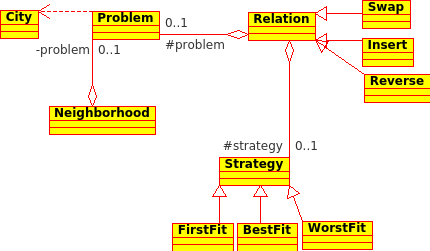
\includegraphics[width=0.6\textwidth,height=0.6\textheight]{../UML/crs.png}
  \end{center}
  
\end{frame}


\begin{frame}
  \frametitle{Phase 1 - Implémentation}
  \framesubtitle{Lancement et mesures préliminaires}
  
  \begin{center}
  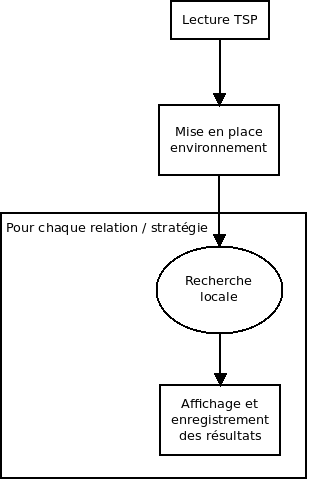
\includegraphics[width=0.6\textwidth,height=0.75\textheight]{images/exec-phase-1.png}
  \end{center}
  
\end{frame}

\begin{frame}
  \frametitle{Phase 1 - Implémentation}
  \framesubtitle{Analyse}
  
  \begin{itemize}
    \item \textbf{Relations de voisinage} :
      \begin{itemize}
	\item Inversion en tête
	\item Échange en dernière position
      \end{itemize}
    \item \textbf{Stratégies d'exploration} :
      \begin{itemize}
	\item Choisir le moins bon améliorant pour des voisinages d'échange et
d'insertion.
	\item Choisir le meilleur améliorant pour un voisinage d'inversion.
      \end{itemize}
  \end{itemize}
  
\end{frame}

\begin{frame}
  \frametitle{Phase 2 - Collecte d'information}
  
  \begin{center}
    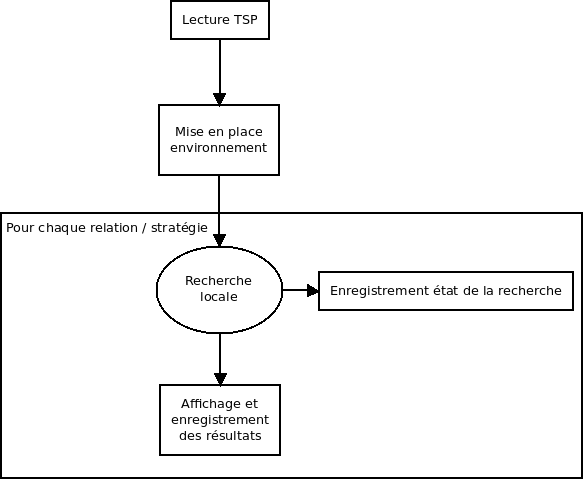
\includegraphics[width=\textwidth,height=0.8\textheight]{images/exec-phase-2.png}
  \end{center}
  
\end{frame}


\begin{frame}
  \frametitle{Phase 2 - Collecte d'information}
  \framesubtitle{Analyse}
  
  Voisinage retenu : \textbf{Reverse}
  
  Comportement en cours d'exécution :
  \begin{itemize}
    \item \textbf{First Fit} : Mouvements erratiques.
    \item \textbf{Best Fit} : De grands mouvements jusqu'à mi-exécution.
    \item \textbf{Worst Fit} : De petits mouvements dès le début.
  \end{itemize}
  
\end{frame}


\begin{frame}
  \frametitle{Phase 3 - Amélioration du système}
  \framesubtitle{Pistes considérées}
  
  \begin{itemize}
    \item Espérance d'amélioration
    \begin{itemize}
      \item Recherche probabiliste
    \end{itemize}
    \item Relations / Stratégies dynamiques
    \begin{itemize}
      \item Changement d'approche en cours de recherche
    \end{itemize}
    \item Algorithmes génétiques
  \end{itemize}

\end{frame}



\begin{frame}
  \frametitle{Conclusion}
  
  \begin{itemize}
    \item Des résultats intéressants pour les voisinages et stratégies étudiées.
    \item Portée réduite par rapport aux prévisions initiales ; laisse sur sa
faim.
    \item Malgré les complications en première partie, projet solide d'un
point de vue technique.
    \item Approche recherche intéressante.
  \end{itemize}

\end{frame}


\begin{frame}
  \frametitle{Remerciements}
  
  Adrien Goëffon, pour avoir aiguillé l'étude de manière efficace et fait
preuve de patience.

  Sara et les étudiants de M2 recherche.
\end{frame}


\end{document}
